\section{Discussion}
%\label{sec:discussion}

In this section, we discuss issues related to parameter selection for our methodology. % (e.g., grid size, number of sectors, and the visualization).
Specifically, we discuss the challenges associated with selecting the appropriate grid size, number of sectors within sub-space, and the visualization.


\subsection{Grid Size}

As discussed in Section~\ref{sec:discretization}, we conducted our evaluations by varying the grid size.
Our evaluation results reveal that the grid size has an impact on the accuracy of the forecast results.
However, selecting an appropriate grid size (i.e., geospatial scale) for analysis remains to be a challenging task.
%
Based on our experiment results, in general, the data with high density is less vulnerable and the accuracy of forecasting with a higher granularity (coarse scale) is higher than that with low granularity (fine scale). 
One adverse case happens when the grid size is 200 meters where we find that the forecast accuracy is worse than that with 500 meters grid size as shown in Figure~\ref{fig:Chart_NRMSE_Grid}.
Interestingly, this is observed in both Twitter and Taxi data.
%[WHY IS THIS NOT SHOWN IN THE IMAGE??]
%Based on our experiment results, we find that the data with high density provide more accurate results.
%We also find that the forecasting performance using finer scales yield better results than that with coarse scales.
%However, the forecast accuracy with 200 meters is worse than that with 500 meters in both Twitter and Taxi data [WHY IS THIS NOT SHOWN IN THE IMAGE??].
%This situation happens to both Twitter and Taxi data.
Although the two datasets have a relatively higher density than the GeoLife data, the overall geospatial densities of the Twitter data are significantly lower.
%However, the datasets have the same geo-boundary as New York City, a big city.
Accordingly, we believe that there may a relationship between the grid size and the geographical characteristics (e.g., demographics) that needs to be further explored.
We leave this as future work.

%=======
%In this work, we conducted experiments with a number of grid sizes and verified that grid sizes highly impact on the forecast results. In addition, we also confirmed that determining the best grid size is challenging. Based on our experiment results, in general, the data with high density is less vulnerable and the accuracy of forecasting with a higher granularity (less grid size) is higher than that with low granularity. One adverse case happens when the grid size is 200 meters--the forecast accuracy is worse than that with 500 meters grid size. Interestingly, we acquired the same result with both Twitter and Taxi data. Although the two datasets have relatively higher density than that of GeoLife data, their densities are also significantly different. However, the datasets have the same geo-boundary as New York City, one of big cities.
%With these results, we think that there could be relationship between the grid size and geographical characteristics, such as a block size in our algorithms.
%>>>>>>> .r9166

\subsection{Number of Sectors}
In our experiments, we investigated the effect of the number of sectors of the flow forecast accuracy. 
With the high density datasets (Twitter and Taxi data), we find that the number of sectors has impact on the forecasting accuracy as shown in Figure~\ref{fig:Chart_NRMSE_Sector}.
We believe that the smaller number of sectors can cause low directional accuracy
since each divided sector covers a larger range of the direction of vectors when the number of sectors is low. Moreover, we believe that the error rates for the number of sectors are also influenced by the degree of freedom for the movement. If there are many possible paths in a geographical location, the larger number of sectors introduce the less errors. Moreover, the orientations of the representative vectors also affect the error rates according to the number of sectors since a representative vector covers an aggregated direction. We will investigate the optimal number of sectors to minimize the errors as a future work. 
%AM: I FIND THESE FINDINGS STRANGE. LETS DISCUSS THIS IN PERSON TO SEE HOW WE CAN EXPLAIN THIS.  

%But, a higher number of sector requires larger computation for forecasting.


\begin{figure}[t]
	\centering
	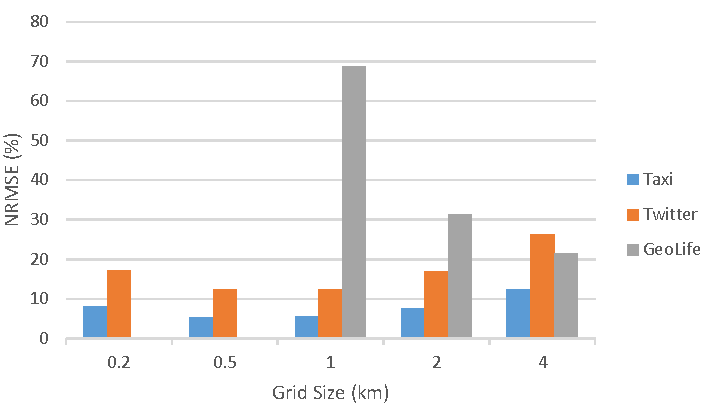
\includegraphics[width=1.0\columnwidth]{Chart_NRMSE_Grid}
	\caption{NRMSE vs the grid size}
	\label{fig:Chart_NRMSE_Grid}
\end{figure}

%\begin{figure}[tbh]
	%\centering
	%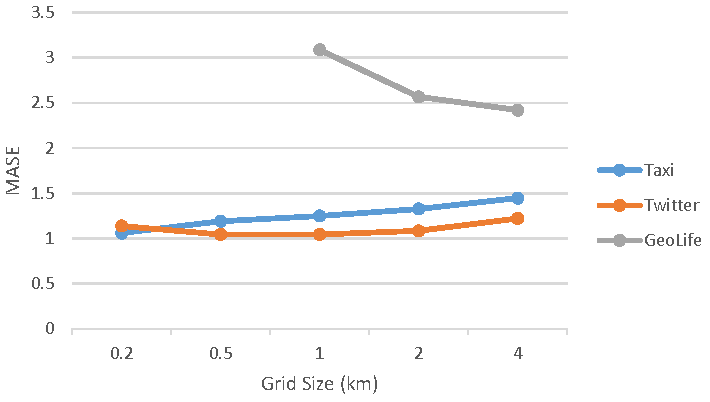
\includegraphics[width=1.0\columnwidth]{Chart_MASE_Grid}
	%\caption{MASE vs the grid size}
	%\label{fig:Chart_MASE_Grid}
%\end{figure}


\subsection{Visualization}
Our flow visualizations are designed to capture the density of each direction. The high density flow is colored in red, while the low density flow is colored in blue. As mentioned in Section~\ref{sec:forecasting-visualization}, the density is treated as the probability of a particle moving toward a direction. As seen in the probability flow in Figure~\ref{fig:twitter_flow}~(B), the low density flow areas tend to have multiple directional uncertain flows, while the high density flow areas have only one or two major certain flows. This indicates that a low density area generates many possible flow paths, but a high density area produces only a few possible flow paths. Therefore, we can differentiate these two flows by the complexity of flow path patterns. Additionally, the major flow provides smoother flows with densities compared to the probability flow. This allows us to observe the overview of the flow vector fields as seen in Figure~\ref{fig:twitter_flow}~(A).

\section{Conclusion and Future Work}

In this paper, we presented a space-based visual analytics approach for forecasting the overall flow of human crowds. 
Our work utilizes individual movement trajectory data and embeds it into a two-dimensional Euclidean space.
Our approach is based on modeling for the space instead of the more conventional approach of modeling individual objects. 
We also propose a new flow smoothing method based on local and global trend estimates in order mitigate for the challenges resulting from data sparseness and noise in the data. 
We utilize the seasonal trend decomposition based on LOESS technique to forecast the future flow using observed historical flow patterns.
We provide several case studies to demonstrate our work. 

Our future work includes factoring in correlations with other datasets in order to further refine our trajectory forecasting methods.
We also plan on incorporating data-driven methods to fragment the geospace based on other features (e.g., road network) instead of only regular grids to compute the forecasts. 
For example, properties of the data may lend themselves well to certain spatial groupings, thereby providing a natural hierarchy for the forecasting. In addition, we will study the influences on the forecasting errors and the optimal forecasting parameters. 
Finally, we plan on further investigating the effects of data sparsity and noise issues on our forecasting results. 


\begin{figure}[t]
	\centering
	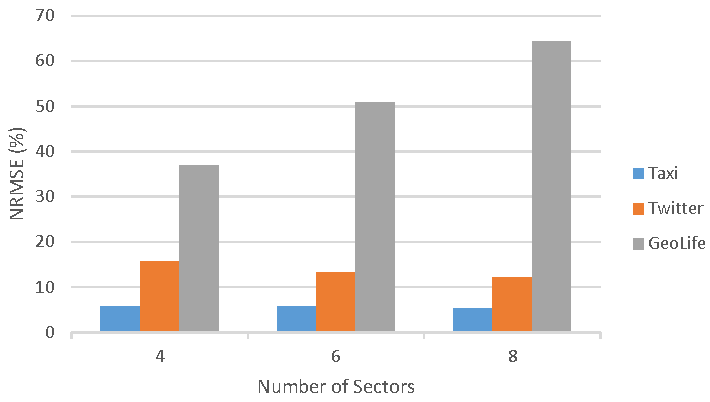
\includegraphics[width=1.0\columnwidth]{Chart_NRMSE_Sector}
	\caption{NRMS vs the number of sectors}
	\label{fig:Chart_NRMSE_Sector}
\end{figure}


